% Fragmento editable: solo TikZ básico, sin bibliotecas adicionales.
% Escala común proporcional: x = índice / 140000.
% Límites exactos: 0, 1/7, 2/7, 6/7, 1.
% Las barras ocupan 0.84\textwidth; los extremos dejan margen para rótulos.
% Los descartes se rotulan fuera de los segmentos cortos, sin reducir letra.
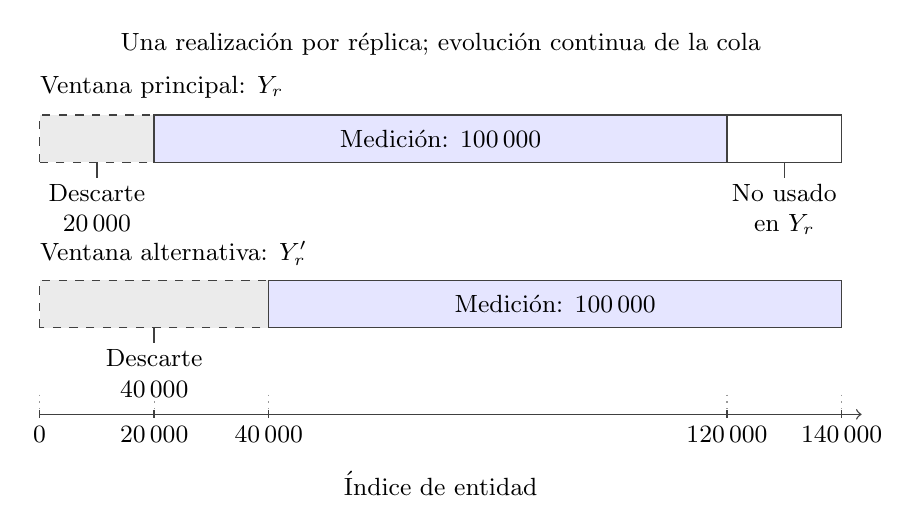
\begin{tikzpicture}[
  x=0.84\textwidth,y=1cm,font=\small,
  borde/.style={draw=black!75,line width=0.5pt},
  descarte/.style={borde,fill=black!8,dashed},
  medicion/.style={borde,fill=blue!10},
  nota/.style={align=center,inner sep=2pt}
]
  \node[nota] at (0.5,2.5)
    {Una realización por réplica; evolución continua de la cola};
  \node[anchor=west,inner sep=0pt] at (0,1.95) {Ventana principal: $Y_r$};
  \path[descarte] (0,1) rectangle ({1/7},1.6);
  \path[medicion] ({1/7},1) rectangle ({6/7},1.6);
  \path[borde,fill=white] ({6/7},1) rectangle (1,1.6);
  \node[nota] at (0.5,1.3) {Medición: $100\,000$};
  \draw[borde] ({1/14},1) -- ({1/14},0.8);
  \node[nota,anchor=north] at ({1/14},0.8) {Descarte\\$20\,000$};
  \draw[borde] ({13/14},1) -- ({13/14},0.8);
  \node[nota,anchor=north] at ({13/14},0.8) {No usado\\en $Y_r$};

  \node[anchor=west,inner sep=0pt] at (0,-0.15) {Ventana alternativa: $Y'_r$};
  \path[descarte] (0,-1.1) rectangle ({2/7},-0.5);
  \path[medicion] ({2/7},-1.1) rectangle (1,-0.5);
  \node[nota] at ({9/14},-0.8) {Medición: $100\,000$};
  \draw[borde] ({1/7},-1.1) -- ({1/7},-1.3);
  \node[nota,anchor=north] at ({1/7},-1.3) {Descarte\\$40\,000$};

  % Proyecciones de los límites sobre un único eje de índices, no temporal.
  \foreach \x in {0,{1/7},{2/7},{6/7},1} {
    \draw[draw=black!40,line width=0.45pt,dotted]
      (\x,-1.95) -- (\x,-2.2);
  }
  \draw[borde,->] (0,-2.2) -- (1.025,-2.2);
  \foreach \x/\valor in {0/0,{1/7}/{20\,000},{2/7}/{40\,000},
      {6/7}/{120\,000},1/{140\,000}} {
    \draw[borde] (\x,-2.15) -- (\x,-2.25);
    \node[anchor=north,inner sep=2pt] at (\x,-2.28) {$\valor$};
  }
  \node[nota,anchor=north] at (0.5,-2.85) {Índice de entidad};
\end{tikzpicture}
